\chapter{Background}
\label{background}

% Parallel computing and software parallelization are vast, complementary and overlapping areas omnipresent across the whole spectrum of hardware. The topics of major importance.

\quad \textit{Parallel computing} and \textit{software parallelization} are vast, overlapping and complementary computer science areas with a history dating back to 1950s. With the advances in semiconductor industry the topics have left the niche of high-end scientific supercomputers and spread to a much wider area spanning across all consumer electronic devices and have become the topics of the major importance.

% Parallel computing and software parallelization are vast, complementary and overlapping areas omnipresent across the whole spectrum of hardware. The topics of major importance.

\quad Nowadays the parallelism is pervasive. Parallel hardware is omnipresent across the whole wide spectrum of computing systems. In order to exploit all the available hardware capabilities the software has to be parallel as well. And thus, every computer scientist and software developer would benefit from having an insight into the area. Nonetheless, the topics are extremely difficult, require a serious time investment and a great deal of knowledge in various subdomains. It is not always realistic to expect from an average programmer to possess such a deep expertise. For that reason we propose a solution aimed at alleviating the challenging task of manual software parallelization. Our solution consists of the two components. We describe them in chapters \ref{assistant} and \ref{frameworks}.

% Background chapter as the point of basic material accumulation. Based on LLNL tutorials!

\quad In this chapter we accumulate and structure the material, which stresses the importance of software parallelization, highlights its challenges, describes the parallel software engineering process and finally lays the ground for our proposed solutions from chapters \ref{assistant} and \ref{frameworks}. We express our special gratitude to Lawrence Livermore National Laboratory (LLNL) \cite{llnl_computing} for their great parallel computing tutorials. We heavily relied on those to prepare the material of this chapter.

% The story line:
%
% Parallel computing importance
% Challenges of software parallelization:
%     automatic
%     manual
%     machine learning based
%     data-centric parallelization problem
% 
%

\quad The background chapter goes as follows. Section \ref{background_importance} stresses the importance of parallel computing and software parallelization in the modern world. There are numerous software parallelization methods and techniques, but all of them run into their specific challenges and problems. Section \ref{background_challenges} highlights the major problems of various software parallelisation methods. First, it presents the challenges of manual and then automatic software parallelization techniques. There have been various experiments and works employing machine learning (ML) based methods for the task of software parallelization. These challenges form the ground for our program loop parallelization assistant solution to grow on. We describe our solution in chapter \ref{assistant}. Then, in section \ref{background_challenges_dcp} we discuss the problem of data structure choice and how it affects the software parallelization. We present a thorough literature review on the topic of Data Centric Parallelization (DCP) dealing with the task of automatic data structure recognition. Our review concludes with that an automatic data structure recognition techniques are still an unsolved grand challenge. Data structures are often inseparable with algorithms the former support. Our computational frameworks grow on the inseparability fact and form the blend of data structures and algorithms. We propose our solution to the problem in chapter \ref{frameworks}. Furthermore, the modern software design and engineering tasks are extremely rich and complex topics. That is true of parallel software engineering as well of course. In sections \ref{background_paradigms} and \ref{background_oop_design_patterns} we talk about imperative, functional and object-oriented programming paradigms, as well as various OOP software design patterns. Our computational frameworks take the best out of their principles and alleviate the task of software architecture design for an average programmer.

\section{The importance of parallel computing}
\label{background_importance}
\quad The parallelism is pervasive and the future of computing is parallel. There are numerous factors which stress the importance of parallelism in the modern computing world.
\begin{description}
\item[Abundance of natural parallelism] The field of High Performance Computing (HPC) has traditionally been concerned with scientific modelling and simulation of various natural phenomena (climate change, fluid flows, etc.). Such systems consist of numerous often independent parts. When we compile a highly parallel algorithm to a serial sequence of CPU instructions or process a huge data set with independent parts sequentially we are artificially constraining a vastly parallel computation to a serial one. Parallelism is not limited to a natural world, instead many algorithms have inherent parallelism in them.
\item[Semiconductor technology advances and power limits] With advances in transistor density it became feasible to design more complicated CPUs. Initially the trend went into deeper pipelines, but running into power limits the industry design shifted towards multi core CPUs and multiprocessor systems. Such systems require of software to mirror the trend and become parallel as well.
\item[Domain inherent parallelism and specialized computations] The areas like computer graphics for instance have a lot of problems that can be processed in a Single Instruction Multiple Data (SIMD) fashion. That naturally led to specialized co-processors like GPUs. The hardware systems grow complex and heterogeneous.
\end{description}

\section{Challenges in Software Parallelization}
\label{background_challenges}
\quad The problem of software parallelization is extremely complex and multi-faceted. There are various approaches to the problem, but all of them have their pros and cons. Although, the process of software parallelization has characteristically been a very manual task, which is time-consuming and error-prone, there are also automatic and machine learning based techniques. In this section we highlight inherent challenges of these approaches. The solution we propose aims to address all of these. 

\subsection{Manual Parallelization Challenges}
\label{background_challenges_manual}
\quad Software parallelization has characteristically been a very manual process. As any software development process it consists of a number of stages and parts. The major problems are described below.
\begin{description}
\item[Problem understanding and partitioning] As the best software engineering practices dictate, before diving into software development one needs to thoroughly understand the problem to be solved and decide on the requirements and restrictions the final piece of software must meet. The whole algorithm and software architecture might change with the decision of developing a parallel software version instead of a serial one. If one starts from an already implemented serial software version, the parallelization might be even more difficult to do. Source code comprehension is a hard task. The algorithm chosen for a serial version might be completely unsuitable for a parallel implementation. The problem must be partitioned into relatively independent chunks of work to be processed in parallel. The partitioning can be done in numerous ways and a programmer needs to choose the way to do that (data set decomposition, functional decomposition or a hybrid of the two).
\item[Communications and synchronization] Very often the parts of the problem to solve are not completely independent and require an exchange of information. Designing the way that exchange is going to work is a complex task. Almost always communication results into an overhead. Sending the data over congested network or waiting on a synchronization barrier all that slows the program down. The slowdown might even diminish all performance benefits obtained from parallelization.
\item[Implementation and data dependencies] When the problem partitioning is done, all communication and synchronization points are determined and the high level parallel algorithm is designed a programmer might start the actual implementation. Here a programmer will run into other types of problems. Consider two functionally equivalent code samples below.\newline\null
\begin{minipage}[t]{0.50\linewidth}
\begin{lstlisting}[caption={Non-parallelizable loop with planted loop-carried data dependence.},label={lst:code_sample_data_dependence},language=C]
for (int i=1; i<n; i++) {
  a[i]=a[i-1]+1;
}
\end{lstlisting}
\end{minipage}
\begin{minipage}[t]{0.50\linewidth}
\begin{lstlisting}[caption={Parallelizable loop free of any data dependencies.}, label={lst:code_sample_no_data_dependence},language=C]
for (int i=0; i<n; i++) {
  a[i]=a[0]+i;
}
\end{lstlisting}
\end{minipage}

The actual shape of the code can break parallelization by introducing fake (not required by the algorithm) dependencies.
\item[Performance analysis and tuning] One needs to know where the program's hotspots are. Hotspots are the places where the most of the real work is being done. The majority of programs spend most of the CPU time in a few places. The task of a programmer is to find those places and concentrate all parallelization and optimization efforts right there. Finding hotspots might be difficult before the programmer has the whole program implemented. Modern hardware architectures have a multi level memory hierarchy, memory data prefetchers, TLBs, out-of-order execution, etc. It might be surprising how the actual program execution performance differs from the one inferred from the algorithm. Profilers and other analysis tools can be of help here.
\end{description}
\quad Finally, all the above challenges are interrelated and very often depend on each other. Parallel software development process can go iteratively with numerous dead ends and redesign efforts. With a long research history into the topic, all these problems are still actual now.

\subsection{Limitations of Automatic Techniques}
\label{background_challenges_automatic}
\quad Given the enormous challenges of manual software parallelization there have been numerous attempts to automate the task. There are various tools available to assist a programmer in the task of software parallelization. Parallelizing compilers are the most widely used ones. Below we present their classification

\begin{description}[noitemsep]
\item[Fully Automatic] The compiler analyzes the source code and identifies opportunities for parallelism.
The analysis includes identifying inhibitors to parallelism and possibly a cost weighting on whether or not the parallelism would actually improve performance. Loops are the most frequent target for automatic parallelization. 
\item[Programmer Directed] Using compiler directives or possibly compiler flags, a programmer explicitly tells the compiler how to parallelize the code. These directives and flags may be also used in conjunction with some degree of automatic parallelization. The most common compiler generated parallelization is done using on-node shared memory and threads (such as OpenMP).
\end{description}
\quad If one is beginning with an existing serial code and have time or budget constraints, then automatic parallelization may be the answer. However, there are several important caveats that apply to automatic parallelization.
\begin{description}[itemsep=0mm]
\item[Correctness] Wrong results may be produced.
\item[Performance] Performance may actually degrade.
\item[Flexibility] Much less flexible than manual parallelization.
\item[Limitations] Limited to a subset (mostly loops) of code.
\item[Effectiveness] May actually not parallelize code if the compiler analysis suggests there are inhibitors or the code is too complex.
\end{description}

\quad To brightly illustrate the problems automatic software parallelization faces we conducted several experiments with the suite of NAS Parallel Benchmarks (NPB). These benchmarks target performance evaluation of highly parallel supercomputers. Consequently, the suite has a great amount of inherent parallelism and is supposed to be easily parallelizable. Indeed, the suite consists of benchmarks based mostly on flat arrays and loop nests operating with them. There are a lot of simple reductions.     



\begin{table}
  \begin{minipage}{\pagewidth}
  \begin{center}
    \begin{tabu}{M{3.0cm}M{1.0cm}M{3.0cm}M{1.0cm}M{3.0cm}M{1.0cm}}
      \hline
      \rowfont{\bfseries}
      reason & num & reason & num & reason & num\\\hline
      \textbf{unrecognised reduction} & 18 & \textbf{array privatization} & 7 & \textbf{AA conservativeness} & 60\\\hline
      \textbf{unknown iteration number} & 7 & \textbf{static dependencies} & 46 & \textbf{too complex} & 22\\\hline
      \textbf{uninlined calls} & 4 & \textbf{other} & 4 & \textbf{total} & 168\\\hline
    \end{tabu}
  \end{center}
  \end{minipage}
  \caption{Classification of loops missed by Intel Compiler for various reasons.}
  \label{tab:icc_missed_opportunities}
\end{table}%

We measured the running time of NASA Parallel Benchmarks after being compiled with Intel compiler (ICC) using various automatic parallelization options. Figure \ref{fig:benchmarks_runtime} illustrates the problems automatic parallelization has.

\begin{figure}[ht]
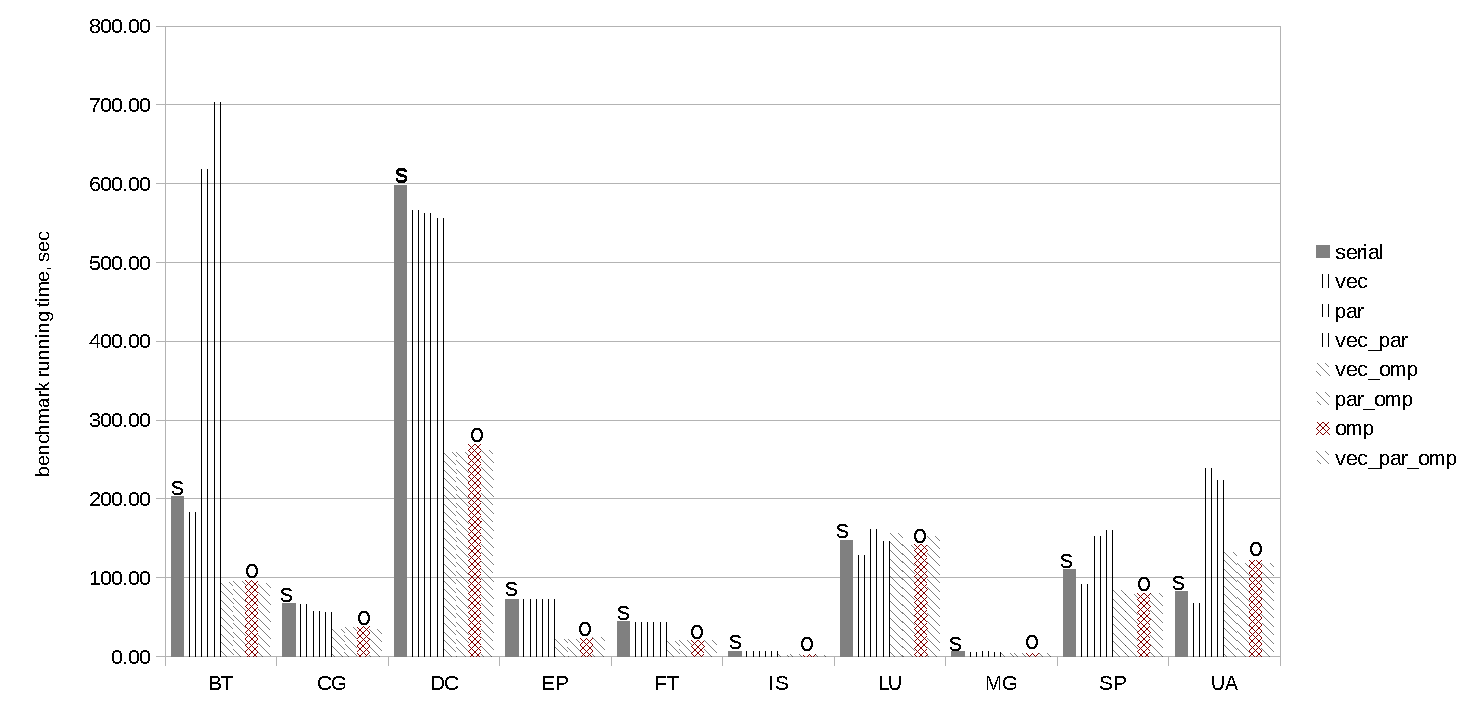
\includegraphics[width=1.0\textwidth]{images/benchmark_runtime.pdf}
\caption{The running time of various NPB benchmarks versions.}
\label{fig:benchmarks_runtime}
\end{figure}

\subsection{Limits of Machine Learning based methods}
\label{background_challenges_ml}
%We focus our discussion of related work on contributions, which are related to the ML aspects of the approach presented in this paper.

\textit{Profitability Analysis.}
The SUIF \cite{Wilson:1994:SIR:193209.193217} parallelizing compiler uses a simple heuristic based on the product of statements per loop iteration and number of loop iterations to decide whether a parallelizable loop should be scheduled to be executed in parallel. In contrast, Tournavitis \emph{et al.}~\cite{Tournavitis:2009:THA:1542476.1542496} use a machine learning based heuristic, which incorporates \textit{dynamic} program features collected in a separate profiling stage, to decide if and how a potentially parallel loop should be scheduled across multiple processors.

\textit{ML in Compiler Optimization.}
Machine learning has been used to solve a wide range of problems, from the early successful work of selecting compiler flags for sequential programs, to recent works on scheduling and optimizing parallel programs on heterogeneous multi-cores. Some works for machine learning in compilers look at how, or if, a compiler optimization should be applied to a sequential program. Some of the previous studies build supervised classifiers to predict the optimal loop unroll factor \cite{4907653,1402082} or to determine whether a function should be inlined \cite{Zhao2003ToIO,1559966}. These works target a fixed set of compiler options, by representing the optimization problem as a multi-class classification problem where each compiler option is a class. Evolutionary algorithms like generic search are often used to explore a large design space. Prior works~\cite{Almagor:2004:FEC:997163.997196,Cooper:2005:AAC:1065910.1065921,Ashouri:2017:MMC:3132652.3124452} have used evolutionary algorithms to solve the phase ordering problem (i.e.\ in which order a set of compiler transformations should be applied).

\textit{Machine Learning and Parallelization.}
Most relevant to the work presented in this paper is the approach of Fried \emph{et al.}~\cite{fried_ea:2013:icmla}. Similar to our approach, Fried \emph{et al.} train a supervised learning algorithm on code hand-annotated with OpenMP parallelization directives in order to approximate the parallelization that might be produced by a human expert. However, we do not rely solely on OpenMP annotations, but we complement our training set with substantially richer data obtained from an aggressively configured parallelizing compiler. While Fried \emph{et al.}~focus on the comparative performance of different ML algorithms, we contribute a practical parallelization assistant capable of ranking loop candidates in their order of merit. Through this we directly enhance programmer productivity in an ML-assisted environment. Similarly to our approach, Hayashi \emph{et al.}~\cite{Hayashi:2015:MPH:2807426.2807429} extracts various program features during compilation for use in a supervised learning prediction model. However, its aim is the optimal runtime selection of CPU vs. GPU execution and it is limited to programs written in Java using the parallel stream APIs that was introduced in version 8.

\subsection{Data-Centric problem}
\label{background_challenges_dcp}
\quad As it has already been stated the problem of software parallelisation is multifaceted. There is a vast range of lower level technical issues, which can turn a perfectly parallelisable at a higher level computation into a non-parallelisable implementation. In our ML assistant project (see Chapter \ref{chapter_ml_assistant}) we showed that the main reasons of Intel Compiler failures on SNU NPB benchmarks are alias analysis conservativeness, uninlined function calls and statically unresolvable dependencies. The assistant tool we designed targets these aspects of the software parallelisation problem. But, there are many more reasons leading to non-parallelisable algorithm implementations. Source code listings \ref{lst:array} and \ref{lst:list} brightly illustrate yet another unsolved problem.\newline\null
\begin{minipage}[t]{0.45\linewidth}
\begin{lstlisting}[caption={Parallelisable loop operating on a \textbf{linear array}.},label={lst:array},language=C]
for (int i=0; i<n; it++) {
  a[i]=a[i]+1;
}
\end{lstlisting}
\end{minipage}
%
\begin{minipage}[t]{0.55\linewidth}
\begin{lstlisting}[caption={Non-parallelisable loop operating on a \textbf{linked-list}.},label={lst:list},language=C]
for (p=list; p!=NULL; p=p->next) {
  p->value+=1;
}
\end{lstlisting}
\end{minipage}
\quad Listings \ref{lst:array} and \ref{lst:list} illustrate two alternative implementations of the same simple computation. We increment all sequence elements by one. Listing \ref{lst:array} implements the sequence with a regular array linearly laid out in the memory. Listing \ref{lst:list} chooses a linked list as an implementing data structure, which leads to a source code non-parallelisability.\newline\null
\quad The DCP problem is not solved. Automatic methods are limited to relatively simple code bases such as libraries of well known data structures. The most successful methods rely on dynamic analysis and mamory graphs. Static techniques such as shape analysis are undecidable and highly conservative and might not finish in a reasonable time for the real software projects. Section [] gives a detailed literature review on the topic. 


\subsection{Parallel Programming Models}
\quad With a number of various hardware and operating system vendors entering the market with their different hardware architectures and system call interfaces software portability became a serious concern.   



To combat the problem industry vendors and major organisation came to design industry standards such as POSIX, OpenMP and MPI. 



\section{Data-Centric Parallelization}


\label{background_dcp}
\subsection{The Problem}
\quad As it has already been stated the problem of software parallelisation is multifaceted. There is a vast range of lower level technical issues, which can turn a perfectly parallelisable at a higher level computation into a non-parallelisable implementation. In our ML assistant project (see Chapter \ref{chapter_ml_assistant}) we showed that the main reasons of Intel Compiler failures on SNU NPB benchmarks are alias analysis conservativeness, uninlined function calls and statically unresolvable dependencies. The assistant tool we designed targets these aspects of the software parallelisation problem. But, there are many more reasons leading to non-parallelisable algorithm implementations. Source code listings \ref{lst:array} and \ref{lst:list} brightly illustrate yet another unsolved problem.\newline\null
\begin{minipage}[t]{0.45\linewidth}
\begin{lstlisting}[caption={Parallelisable loop operating on a \textbf{linear array}.},label={lst:array},language=C]
for (int i=0; i<n; it++) {
  a[i]=a[i]+1;
}
\end{lstlisting}
\end{minipage}
%
\begin{minipage}[t]{0.55\linewidth}
\begin{lstlisting}[caption={Non-parallelisable loop operating on a \textbf{linked-list}.},label={lst:list},language=C]
for (p=list; p!=NULL; p=p->next) {
  p->value+=1;
}
\end{lstlisting}
\end{minipage}
\quad Listings \ref{lst:array} and \ref{lst:list} illustrate two alternative implementations of the same simple computation. We increment all sequence elements by one. Listing \ref{lst:array} implements the sequence with a regular array linearly laid out in the memory. Listing \ref{lst:list} chooses a linked list as an implementing data structure, which leads to a source code non-parallelisability.\newline\null
\quad In the project of "Data-Centric Parallelisation (DCP)" we would like to automatically recognise 
\subsection{Literature Review}
\label{background_dcp_literature_review}
\quad The idea of automatic discovery of higher level entities in programs is not a new one. This discovery problem is closely interlinked and entangled with alias analysis techniques \cite{Muchnick:1998:ACD:286076} like points-to analysis \cite{Emami:1994:CIP:178243.178264}. Points-to analysis is a variation on data flow analysis techniques. The final output is the sets of pairs of the form (\textit{p},\textit{x}) (pointer variable \textit{p} points to a stack allocated variable \textit{x}). These techniques are aimed at getting aliasing information regarding stack-allocated pointers.\newline\null
\quad The problem of understanding heap-directed pointers and heap-allocated linked data structures these pointers might point to is addressed with a family of static analysis techniques collectively known as shape analysis. Shape analysis techniques can be used to verify properties of dynamically allocated data structures in compile time. These are among the oldest and most well known techniques. Three-valued logic \cite{Sagiv:1999:PSA:292540.292552}\cite{Wilhelm:2000:SA:647476.760384} can be used as an example. The technique proposes a construction of a mathematical model consisting of logical predicate expressions. The latter correspond to certain pointer operating imperative language program statements. Abstract interpretation of these statements leads to a construction of sets of shape graphs at various program points. Shape graphs approximate the possible states of heap-allocated linked data structures and answer the questions such as node reachability, data structure disjointness, cyclicity, etc. The major limitation of these simplified mathematical models is the lack of precision high level of abstraction leads to. The problem of precise shape analysis is provably undecidable.\newline\null
\quad The work of \cite{Ghiya:1996:TDC:237721.237724} proposes a simplified and hence more practical implementation of shape analysis. Authors propose to use direction \textit{D} and interference \textit{I} matrices instead of complex mathematical models in order to derive shape information on heap allocated data structures. The entry of direction matrix \textit{D[p,q]} says if there exists a path from a node referred to by \textit{p} to a node referred to by q. In other words, if we can enter a path withing the data structure through \textit{p} and exit through \textit{q}. The entry of interference matrix \textit{I[p,q]} says if the paths started from \textit{p} and \textit{q} are going to intersect at some point. Authors implement their technique withing McCAT compiler, which uses SIMPLE intermediate representation with a total of 8 statements (\textit{malloc()}, pointer assignments \textit{p=q}, structure updates \textit{p-$>$next=q}), which are capable of changing \textit{D} and \textit{I} matrices. Statements generate and kill entries in matrices. Moreover, they are capable of changing \textit{Shape} attribute of pointers. The technique has been assessed on various benchmarks (bintree, xref, chomp, assembler, loader, sparse, etc.) from the era before the standard benchmark suites became available. The technique mostly reported shapes as \textit{Trees} (be it a binary tree or a linked-list) or sometimes as \textit{DAGs} or \textit{Cycles} but with higher error rates in these last cases. The latter shows that the technique is imprecise and conservative.\newline\null
\quad One of the more recent techniques designed and developed by Philip Ginsbach and Michael F. P. O’Boyle is based on the pattern matching on LLVM IR level. The main idea is to specify computational idioms to be recognized in a domain specific constraint based programming language CAnDL \cite{Ginsbach:2018:CDS:3178372.3179515}. Constraints are specified over LLVM IR entities such as instructions, basic blocks, functions, etc. The CAnDL language allows for a rapid prototyping of new compiler optimisations based on pattern recognition and its substitution with an optimised versions of matched idioms. The language and its relatively fast backtracking constraint solver are capable of recognizing not only simple arithmetic idioms (thus performing different peephole optimizations), but more complex computations like general reductions and histograms \cite{Ginsbach:2017:DEG:3049832.3049862}, vector products in graphics shaders \cite{Ginsbach:2018:AML:3296957.3173182}, sparse and dense linear algebra computations and stencils \cite{Ginsbach:2018:AML:3296957.3173182}. Having recognized these computational idioms the work \cite{Ginsbach:2018:AML:3296957.3173182} replaces them with a code for various heterogeneous APIs (MKL, libSPMV, Halide, clBLAS, CLBlast, Lift) and compares the resulting performance demonstrating an improvement over sequential versions and matching performance to a hand-written parallel versions. The technique has been deployed on the sequential C versions of SNU NPB, the C versions of Parboil and the OpenMP C/C++ versions of Rodinia demonstrating an improved detection capabilities over the state-of-the-art techniques.\newline\null
\quad The other principally different technique has been recently proposed by Changhee Jung and Nathan Clark \cite{1669122}. The authors developed a Data-structure Detection Tool (DDT) based on LLVM framework. The tool instruments loads, stores and calls withing program binaries and gathers dynamic traces for sample inputs. The traces are used to recreate a memory allocation graph for program data structures. Call graphs are used to identify interface functions interacting with the built memory graph. DDT traces memory graph properties (number of nodes, edges, etc.) before and after interface function calls into another Daikon tool to compute dynamic invariants (the number of nodes in a memory graph decreses by 1 after every \textit(delete()) interface method call, etc.). At the end manually constructed decision tree is used to probabilistically match observed behavioral patterns against known data structure invariant properties. The technique has been deployed to recognise data structure implementations withing standard libraries like STL, Apache (STDCXX), Borland (STLport), GLib, Trimaran achieving almost perfect recognition accuracy. Moreover, the technique has been able to recognise linked lists in Em3d and Bh Olden benchmarks, along with red-black trees implementing vectors in Xalancbmk benchmark.\newline\null
\quad There has recently been other published works on the application of dynamic techniques to the problem of dynamic data structure recognition \cite{Rupprecht:2017:DID:3155562.3155607}\cite{Haller:2016:SDS:2938006.2938029}. The technique used in the DDT tool \cite{1669122} makes an assumption, that all modifications and interactions with memory graphs representing data structures happen through a set of interface functions. That is not true, when we deal with aggressively optimising compilers, which may eliminate some code or inline some functions. The MemPick tool \cite{Haller:2016:SDS:2938006.2938029} searches data structures directly on a built dynamic memory graph by analyzing its shape. The graph is built with the help of Intel Pin binary instrumentation tool during quiescent periods, when pointer operations are absent. DSIbin tool \cite{Rupprecht:2017:DID:3155562.3155607} operates with the source code rather than program binaries. Instead of memory points-to graphs it uses strands as primitives, which abstract such entities as singly-linked lists.\newline\null
\quad The work of Dekker \cite{Dekker:1994:ADS:3107859.3107876} addresses software design recovery problem in a completely different way. Contrary to the approaches described above, which operate on the IR and dynamic instruction stream levels, work of Dekker operates at the level of abstract syntax tree. Dekker's tool tries to compact the tree down to a recognizable syntactic patterns by transforming it in accordance to a special grammar.


\section{Imperative and Functional programming}
\label{background_programming_paradigms}
\quad Programming languages can be classified by different \textit{programming paradigms} they support. Among the most general classifications are \textit{imperative} and \textit{declarative} programming languages.\newline\null
\quad Imperative programs are written in a form of instruction sequences, which read and write the \textit{state} of a program. The concept of state is the main characteristic of imperative programming paradigm. Instruction sequences can be structured in various ways. In \textit{procedural} programming paradigm instructions are grouped inside procedures and functions. In \textit{object-oriented} programming (OOP) paradigm instructions are grouped with the data they operate on inside objects of various types or classes. Programs are either out of various procedures calling each other and exchanging the data or on the interaction of objects of various types.\newline\null
\quad Declarative programs do not specify the exact sequence of steps and state updates a program needs to do in order to get the desired result. Declarative programs declare the properties of the desired result. The properties can be specified as a set of constraints like in \textit{constraint} programming or a set of linear inequalities like in \textit{linear} programming. \textit{Functional} programming is another subtype of declarative programming. In functional programming the final result is specified as a sequence of stateless function evaluations, which form a tree of expressions. Among the most common constituents are functions like \textit{map}, \textit{reduce}, \textit{fold}, etc. Functions can be passed as arguments and returned from other functions ultimately composing bigger programs.\newline\null
\quad Functional programming is sometimes treated as synonymous with purely functional programming, a subset of functional programming which treats all functions as deterministic mathematical functions, or pure functions. When a pure function is called with some given arguments, it will always return the same result, and cannot be affected by any mutable state or other side effects. This is in contrast with impure procedures, common in imperative programming, which can have side effects (such as modifying the program's state or taking input from a user). Proponents of purely functional programming claim that by restricting side effects, programs can have fewer bugs, be easier to debug and test, and be more suited to formal verification.\newline\null
\quad There are no universally optimal programming paradigms and languages. Some languages are more convenient and suitable for one sort of problems, some languages are better at tackling other problems. For example, functional languages are more convenient in addressing certain domains such as R for statistics and financial analysis. Imperative languages are certainly better for simulations and other state based scientific computations. For that reason, major languages are often multi-paradigm to cover a potentially larger set of problems. Largely imperative C++ language included support for functional programming with its newer standards starting from C++11.\newline\null
\quad Although, there is still the gap. Some problems contain computations, which are better expressed with standard functional concepts, but at the same time require some state keeping. These problems lie at the boundary of functional and imperative programming. Both paradigms are equally important. In the chapter \ref{computational_frameworks} we propose an idea of \textit{computational frameworks}, which fills that gap. 

\section{OOP and Software Design Patterns}
\label{background_oop_design_patterns}
\subsection{Object-Oriented Programming (OOP)}
\label{background_oop}
\quad Object-oriented programming (OOP) is arguably the most widely used programming paradigm nowadays. It is supported by almost all major programming languages. At the very essence, in OOP computer programs are designed by making them out of objects that interact with one another. Object interactions are very close to human level of reasoning and logic and thus the paradigm fits quite naturally to a human developer.\newline\null
\quad Objects are instances of different types or classes in OOP terminology. Classes are object specifications. They specify the data objects contain (like an integer \textit{age} field for an object of class \textit{Person}), the methods used to operate on the data. Classes define the public part of objects as well as their internal implementation. Object-oriented languages provide a rich set of facilities and fatures to build programs. The major are described below.\newline\null
\quad \textit{Encapsulation} is another OOP technique, that is used for protection against object misuse and unintended outside interference. Data and methods of a class concerned with its internal workings are declared \textit{private} to a class, while those designed to form an outward appearance and interface of a class are declared \textit{public}. This facilitates code refactoring, for example allowing the author of the class to change how objects of that class represent their data internally without changing any external code. It also eases a program comprehension and debugging by better localizing functionality and thus possible bugs.\newline\null
\quad \textit{Dynamic dispatch} is the responsibility of the object, not any external code, to select the procedural code to execute in response to a method call, typically by looking up the method at run time in a table associated with the object. This OOP feature allows a programmer to write a more general code, which works with abstract interface methods and leave the exact method resolution to be made during the running time of a program.\newline\null
\quad The technique of a dynamic dispatch is closely related to the technique of \textit{inheritance}. Inheritance allows classes to be arranged in a hierarchy that represents "is-a-type-of" relationships. Inheritance can be of two types: interface inheritance and implementation inheritance. The first one allows a parent class to require its descendants to stick to the same interface. A common interface allows the objects of different classes from the same hierarchy to be operated on by the same type agnostic code. The latter is called a \textit{polymorphism}. The user code can be more concise and abstract. The call of the same method on the parent class or one of its descendants can result into a varying behaviour.
\subsection{Software Design Patterns}
\label{background_design_patterns}
\quad The presence of all the above features makes OOP languages extremely rich with various facilities. That creates a vast design space for software architects and engineers and spawns the whole topic of software design patterns.  

\quad Software design patterns are reusable solutions to common design problems in object-oriented software engineering. They live at the level higher than that of a source code and are language agnostic. The solutions can be regarded as standard solutions to design problems they target. These solutions have been well tested and proven to be the most reliable and elegant.

\quad At the end it is the experience, mastery and ingenuity of a programmer which determine the final software design.  

\subsection{Computational frameworks as design patterns }
\label{background_design_patterns_frameworks}
\quad Our computational frameworks embody all the above concepts and principles and are based on modern and convenient software design patterns. Our frameworks free a programmer from a complex process of a software design.  

Chain of responsibility pattern is very similar to fold.
Visitor pattern roughly corresponds to fold.

\section{Parallel Algorithmic Skeletons}

\section{Benchmarks Studies}
\label{background_benchmarks}
\quad In our projects we used three benchmark suites. We trained our machine learning based loop parallelization assistant with Seoul National University's implementation of the NASA Parallel Benchmarks (NPB) \cite{snu-npb-benchmarks}. For the data-centric parallelization project we started with the SPEC CPU2006 benchmarks. The complexity of these and the perspective we derived for the SPEC CPU2006 suite study led us to a simpler suite of Olden benchmarks. We used the latter for the project of computational frameworks.\newline\null
\quad Below we provide descriptions of the benchmarks so a reader can develop a better feel for the problems we tackle and the code we work with.\newline\null
\subsection{NASA Parallel Benchmarks (NPB)}
\label{background_benchmarks_npb}
\quad NAS Parallel Benchmarks (NPB) target performance evaluation of highly parallel supercomputers. There are 10 various benchmarks in the suite. Benchmarks perform various scientific computations. They solve various systems of linear equations, compute gradients, work with matrices (compute matrix transpose, inverse, etc.), solve differential equations, solve heat and diffusion equations on the mesh, compute 3d grids, but all of them work with the simplest flat arrays at the very core.  


NPB benchmarks only specify the computation to be done, but do not provide the actual implementation. We used the implementation from Seoul National University (SNU NPB).

These scientific computations posses an enormous amount of inherent parallelism in them, but surprisingly run slower after the automatic parallelization as our experiments from the section \ref{background_challenges_automatic} showed. 


Our loop paralleization assistant 

Indeed, the suite consists of benchmarks based mostly on flat arrays and loop nests operating with them. There are a lot of simple reductions.    



\subsection{SPEC CPU2006}
\label{background_benchmarks_spec}
\quad The project of Data-Centric Parallelization (DCP) started with the feasibility studies of the SPEC CPU2006 benchmark suite. We studied the feasibility of the automatic data structure recognition techniques on these benchmarks. Although the benchmarks proved to be extremely complex for such techniques, these studies directed our further efforts and ultimately led to the concept of computational frameworks being an inseparable blend of data structures and algorithms. The key lessons we learnt from the SPEC CPU2006 benchmarks are an enormous complexity of the real legacy code and a very close relationship between data structures and algorithms. Let alone automatic techniques, it might take some weeks for an expert engineer to understand what a single benchmark is actually doing. Below we describe some of the benchmarks we looked at.
\paragraph{429.mcf} The benchmark operates with a complex network of nodes and arcs linearly allocated on the heap memory. Despite the simplicity of allocation, every node and arc has numerous pointers forming several object linking chains. Pointers are set in different places withing the source code base (during allocation as well as during consecutive network structure updates), making the deduction of the actual data structure type a task of the grand complexity. The network forms some sort of a spanning tree with several properties true of its nodes: every node has only one child pointer and if a node has several children, then the latter are connected through sibling pointers starting from the first child.\newline\null
\quad\textbf{The tree data structure presents a high interest from the point of its recognition. But even a manual source code analysis and transformation requires a serious effort. Static automatic techniques seem infeasible, while dynamic ones seem to be a grand challenge.}
\paragraph{456.hmmer} Searches a DNA sequence database given a Profile Hidden Markov Model (HMM). The benchmark uses Viterbi algorithm. The implementation works with four dynamic programming matrices allocated linearly as arrays. Algorithm walks either horizontally or diagonally along these matrices and computes reductions of maps. The computation is parallelizable and there has been successful works \cite{Ganesan:2010:AHG:1854776.1854844}\cite{inria} doing it manually for the specialized hardware.\newline\null
\quad\textbf{Despite the complexity of its core function \textit{P7Viterbi()}, the benchmark presents a very high interest for the application of our computational frameworks. Reductions of maps perfectly fit the purpose. We view it as a future work.}
\paragraph{400.perlbench} This benchmark is a cut-down Perl interpreter, which implements the regular expression matching state machine. The benchmark processes the bitcode of a compiled regular expression instruction by instruction. Although, instructions have the same size and are laid out linearly in memory, there might be branches and the whole processing happens in a linked-list offset directed fashion. That requires sequential execution and is far beyond the capabilities of any existent techniques.
\quad\textbf{The benchmark is neither parallel nor a simple one. It makes no point to apply any recognition techniques here.}
\paragraph{470.lbm} The benchmark implements a Lattice Boltzmann Method (LBM) and is a relatively simple one (around ~1400 LOC). The main underlying data structures our benchmark works with are the two 3D grids mapped onto a linear array space, which simulate incompressible fluids in 3D. The benchmark runs a specified number of time steps. During each time step the benchmark linearly runs along \textit{Src} array. Every array element represents a point from a 3D grid and consists of a number of velocity vector projections (South, North, East, West, Top, Bottom,  ... , South-East, etc.) at this point. The values of these projections are being combined and mapped in a stencil fashion onto adjacent elements of independent \textit{Dst} array. The computation is highly parallel and corresponds to a sweeping of \textit{xy} planes (one plane after another) along \textit{z} axis. The benchmark has already been parallelised with an OpenMP pragma in a per element fashion. This benchmark could potentially be used for the discovery of stencil computational idioms. Linear arrays being used in the benchmark do not represent a huge amount of interest from a data-centric point.\newline\null
\quad\textbf{The benchmark operates with 3D grids laid out on regular arrays. The latter do not present a great deal of interest from the point of data structure recognition. It would be interesting to try to recognize an algorithmic stencil.}

\subsection{Olden}
\label{background_benchmarks_olden}
\quad Although our studies of SPEC CPU2006 benchmarks have proved their enormous complexity for the task of automatic data structure recognition, we have managed to get a good perspective and narrow our research path to a much simpler suite of Olden benchmarks. Computations and algorithmic patterns present in Olden benchmarks have ultimately led us to the concept of computational frameworks.\newline\null
\quad Olden benchmark suite consists of 10 benchmarks. For our project we looked at 6 of those (bisort, health, perimeter, treeadd, mst and tsp benchmarks). The nature of different Olden benchmarks varies. Benchmarks health, treeadd and perimeter perform essentially the same computational pattern, but for different problems. We call that pattern a fractal. The latter is a computational framework, i.e the blend of a parallelizible algorithmic skeleton and a tree-based data structure. Different tree branches are being processed independently. Benchmarks tsp and mst solve 2 well-known graph problems namely travelling salesman problem and minimum spanning tree. The other 4 benchmarks perform scientific numerical computations and are bigger, more complex and less interesting from the point of data structure recognition.
\paragraph{bisort}
\textit{\textbf{Definition} A sorted sequence is a monotonically non-decreasing (or non-increasing) sequence. A bitonic sequence is a sequence with $x_{0} \leq ... \leq x_{k} \geq ... \geq x_{n} - 1$ for some k, or a circular shift of such a sequence.}\newline\null
\quad The sequence is based on a binary tree implementation (recursive calls to left and right subtrees). The algorithm is based on a sorting comparator network consisting of several layers. The network can be and is implemented in a divide and conquer way similar to that of a well-known merge sort. Sort() function is called on the left and right array halves recursively. The merging step of the merge sort algorithm is substituted with compare-and-swap step. The latter is possible due to input sequences required to be bitonic.
\quad\textbf{The benchmark is heavily based on pointers, tree swaps and rotations. It presents an interest from the point of divide and conquer algorithm recognition. Static techniques are unlikely to handle the legacy source code of that complexity and style. Dynamic techniques might be able to see the binary tree.}

\paragraph{health} The most promising of all Olden benchmarks. Columbian health care system simulation is based on a complete 4-ary tree of $4^{max\_level}$ adjacent villages. Each village has its own hospital and is connected to 4 adjacent child villages. Simulation starts from the top (tree root village and goes down all the tree branches recursively right to left.
Every simulation step consists of several stages:
\begin{enumerate}
  \item Accept all patients from adjacent villages and put them in the local hospital for an initial assessment and possibly for further hospitalization inside the local hospital.
  \item Check patients who are inside the local hospital: once inside patients spend time to recover and occupy 1 member of the staff throughout all time. If time have passed then the patient is checked out and releases 1 personnel member.
  \item Check patients on the assessment list. Patients require some time to be diagnosed. Each patient occupies 1 member of the staff throughout the whole assessment process. If patient is ill then he continues to occupy the same personnel member and goes inside the hospital. If patient is healthy then the patient is checked out and releases 1 staff member.
  \item Check patients on the waiting list. Once a patient gets into the hospital he/she takes on 1 member of the staff if the personnel is available. If not, then the patient goes onto the waiting list. Patient passes through 2 phases: assessment and hospitalisation. Each patient is being supervised by 1 member of the personnel starting from assessment and up until checking out of the hospital. If after assessment a patient turns out to be healthy then the patient is checked out and a personnel member is returned back to available pool. If patient is confirmed ill, then the former is put inside the hospital and spends time there. Patients fall ill at the will of a random number generator.
\end{enumerate}

\textbf{The benchmark operates with quad tree structures and does it in a highly parallel fashion. In our work we call that pattern a fractal. The latter is a computational framework, i.e. the blend of an algorithm and a data structure. The whole structure can be aimed at for an automatic recognition (not just a separate tree or an algorithmic skeleton, but both) even with static techniques.}

\paragraph{perimeter} The benchmark computes the perimeter of a ring (R=2048, r=1024). The ring is mapped onto a grid of elements by painting all the grid elements inside the ring ($r^{2} < x*x + y*y < R^{2}$) as black and all grid elements outside of it as white. Then the grid is being traversed in two different (implementation dependent) ways and detects all flips of color (black to white and vice versa) to sum them up into the final perimeter approximation. The grid is implemented as a quad tree based fractal. The initial square is split into 4 parts (northwest, northeast, southwest, southeast), which in their turn split further on. The process reminds the fractal framework from the health benchmark.  

\paragraph{power} The second by importance is the power pricing computation benchmark. The benchmark is based on a composite structure of C arrays and pointer-based linked lists of various objects such as Root, Laterals, Branches and Leaves. Figure \ref{fig:power_benchmark} illustrates the data structure. The algorithm is basically composed of folds and reductions. C arrays are reduced and linked lists are folded. The algorithm works recursively and starts with the Root::compute() call. The method accumulates power demand
Demand(P,Q) from all lists of Laterals. Accumulation starts with the end of each list. Each lateral accumulates its power demand from all its branches and the latter in turn accumulate power demand from all their leaves. The leaves call
optimize\_node() method, which does a chunk of scientific computations (gradients, vectors, etc.), which compute P and Q. Finally, Root::compute() is called iteratively from a while
loop of power\_pricing\_problem(). Iteration continues up until P and Q error becomes less than the required epsilon. 
\begin{figure}[ht]
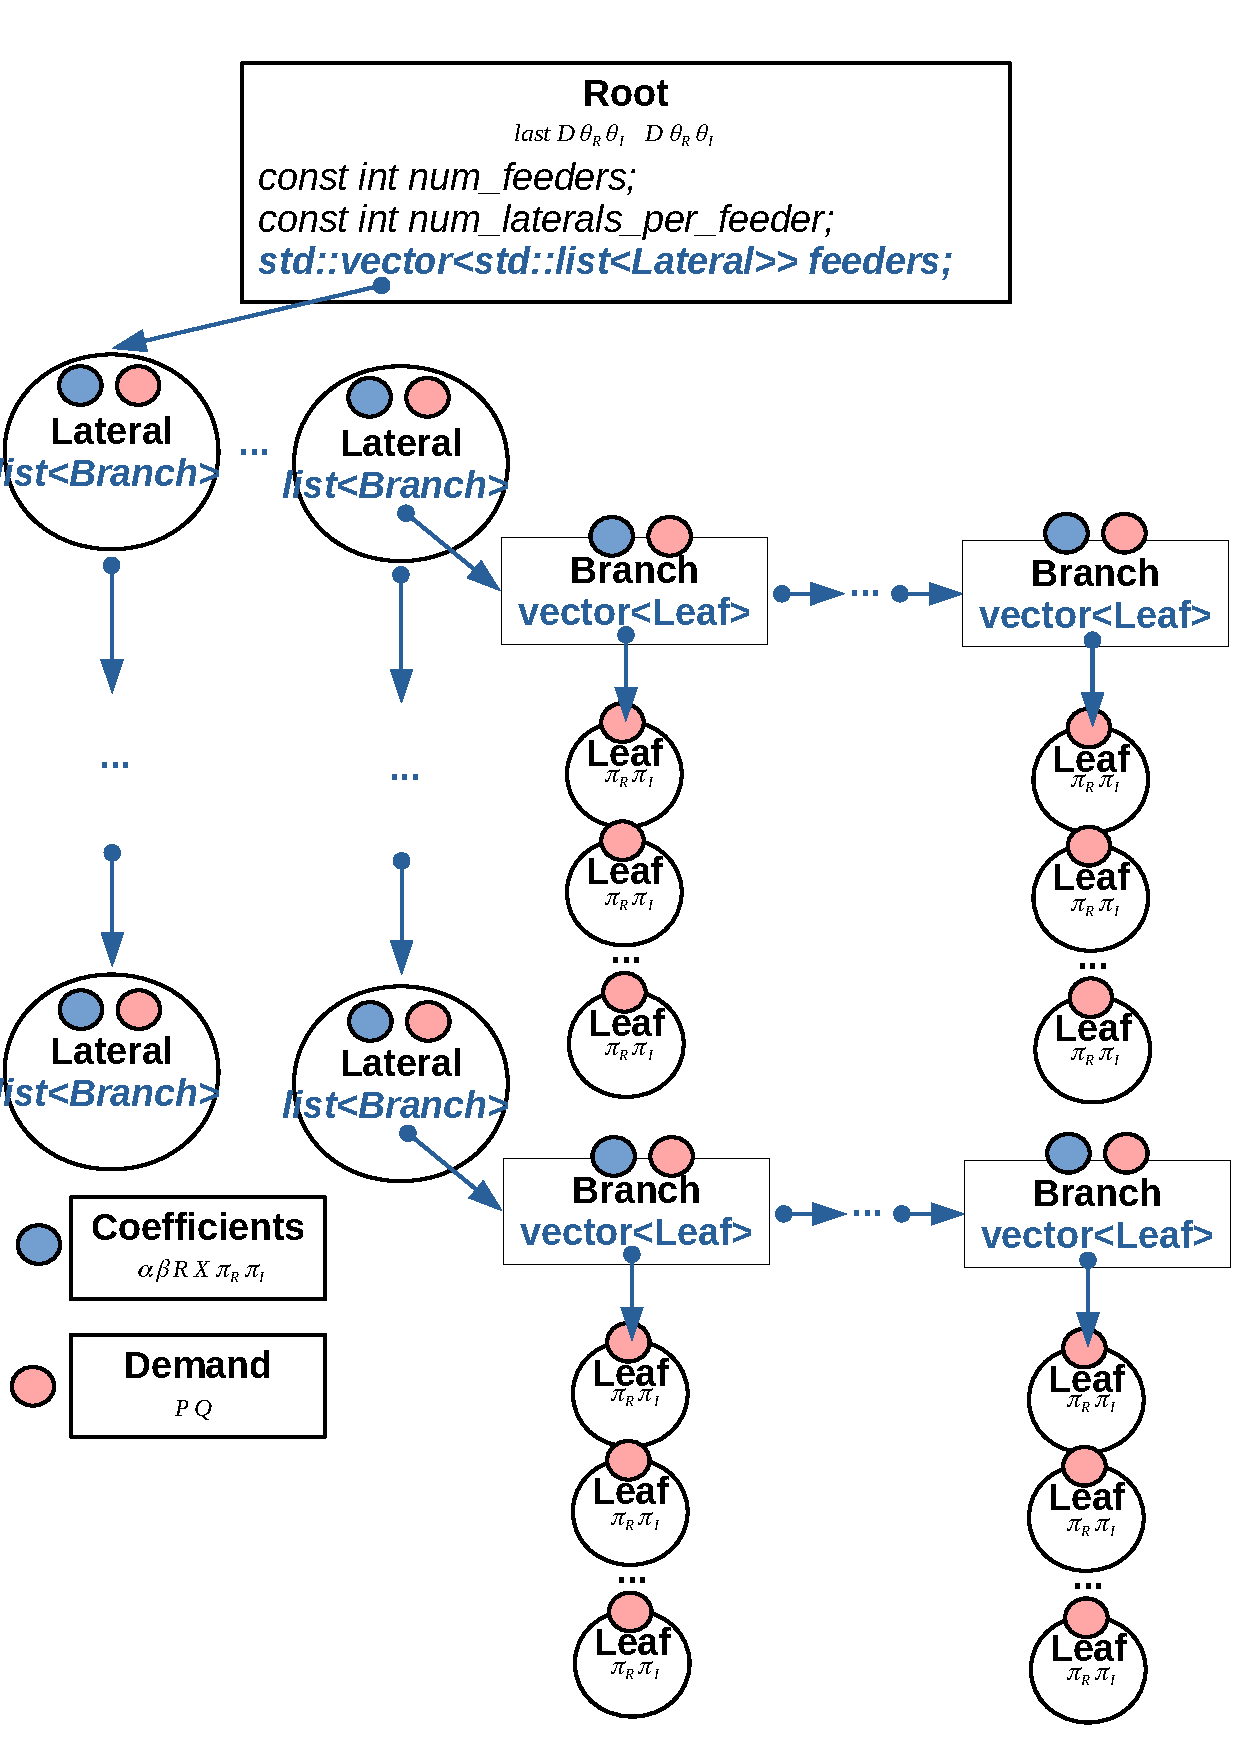
\includegraphics[width=1.0\textwidth]{images/power_scheme.pdf}
\caption{The Power benchmark.}
\label{fig:power_benchmark}
\end{figure}

\paragraph{treeadd} The treeadd benchmark is a very small and simple one. It does a recursive reduction on a pointer-linked binary tree. To create a workload the reduction is done repetitively inside the loop.   

\paragraph{mst} Minimum Spanning Tree (MST) benchmark does a MST weight computation of a complete graph. Computation is approximate and the algorithm looks like it might finish with incorrect result. Nevertheless, the benchmark can be used for the purpose of computational workload. Graph is represented as a linked list of vertices. Every node in the list has a hash table of incident edges. Graph is complete: each vertex is connected to all other vertices in the graph (except itself). Algorithm repeatedly traverses the list of vertices and gradually accumulates the MST weight. On every traversal algorithm picks the node in the list to use as an input for the next traversal. In that sense, there is a cross iteration/traversal dependency. The code below summarises the benchmark.\newline\null
\begin{minipage}[t]{\linewidth}
\begin{lstlisting}[caption={The main algorithm of mst benchmark.},label={lst:mst_code},language=C]
vertex = list;
list = list->next;
while (num_vertices) {
    ret = traverse_vertex_list(vertex, list);
    mst_weight += ret.distance; // accumulate the final result
    vertex = ret.vertex; // next vertex to measure the distance against
    num_vertices--;
}
return mst_weight;
\end{lstlisting}
\end{minipage}

\paragraph{tsp} Travelling Salesman Problem (TSP). The benchmark generates a set of dots scattered on a 2D plane. Dots represent cities and are specified by their (x,y) coordinates. The TSP problem is to visit all the cities and return to the city of origin having passed the minimal distance. In other words, the algorithm returns a cycled sequence of cities, where proximity of elements in the sequence in terms of order means their spatial proximity on the 2D plane.\newline\null
\quad The algorithm’s work resembles that of an insertion sort. The sequence is divided into 2 parts. Ordered part and unordered part. At first, ordered part consists of just 1 element. On every iteration the algorithm takes the next element out of unordered part, finds it a pairing element inside the ordered part (with the minimal distance between them) and inserts the element into the ordered subsequence next to its pair. At the end we get the sequence with the property that closest dots stand the closest in the sequence.\newline\null
\quad The benchmark is based on a binary tree being transformed into doubly linked list. Every node of the tree represents a city located on 2D plane with randomly generated (x,y) coordinates. The build\_tree() method is written in a way to generate a uniform distribution of dots on the plane.





